\documentclass{article}
\usepackage[utf8]{inputenc}
\usepackage{amsmath}
\usepackage[parfill]{parskip}
\usepackage{geometry}
 \geometry{
 a4paper,
 total={170mm,257mm},
 left=30mm,
 top=30mm,
 }
 \usepackage{graphicx}

\title{Assignment 1 ( ICSE Class 10 2018 )}
\author{Vedant Bhandare\\CS21BTECH11007}
\date{March 2022}

\begin{document}

\maketitle

\section*{QUESTION}
The circumference of the base of a cylindrical vessel is 132 cm and its height is 25 cm. Find the

\begin{enumerate}
    \item radius of the cylinder
    \item volume of cylinder.(use $\pi = \frac{22}{7}$)
\end{enumerate}

\section*{SOLUTION}

\vspace{2mm}

Let $r$ and $h$ be the radius of the base and height of the cylindrical vessel, respectively.\\
Let $C_{base}$ be its base circumference and $V$ be its volume.\\

We know that,

\begin{center}
    \large{$C_{base} = 2\pi{r}$}
    
    \vspace{2mm}
    
    $V = \pi{r^2h}$
\end{center}

\vspace{2mm}

\subsection*{1. radius of the cylinder}

\vspace{2mm}

\large{$C_{base} = 2\pi{r}$}

\vspace{1mm}

$132 = 2\pi{r}$

\vspace{1mm}

$132 = 2\times\frac{22}{7}\times{r}$

\vspace{1mm}

$r = 21$

\begin{center}
    \large{Thus the radius of base of the cylindrical vessel is $21 \hspace{1mm}cm$.}
\end{center}

\vspace{2mm}

\subsection*{2. volume of the cylinder}

\vspace{2mm}

$V = \pi{r^2h}$

\vspace{1mm}

$V = \frac{22}{7}\times21^2\times25$

\vspace{1mm}

$V = 34650$

\vspace{1mm}

\begin{center}
    \large{Thus, the volume of the cylindrical vessel is $34650 \hspace{1mm} cm^3.$}
\end{center}

\clearpage

\begin{figure}[h]
    \centering
    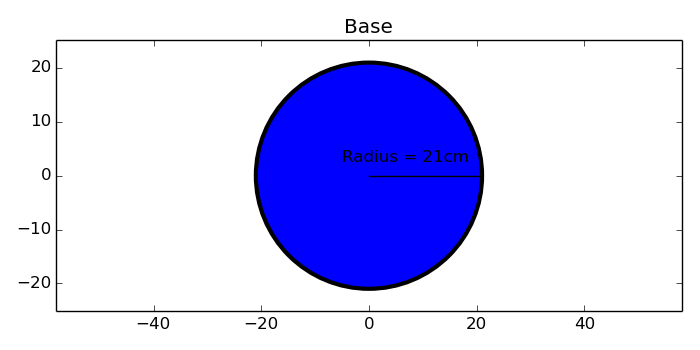
\includegraphics[scale = 0.5]{Figures/Base.png}
    \caption{Base of the cylindrical vessel}
    \label{fig:Base}
\end{figure}

\begin{figure}
    \centering
    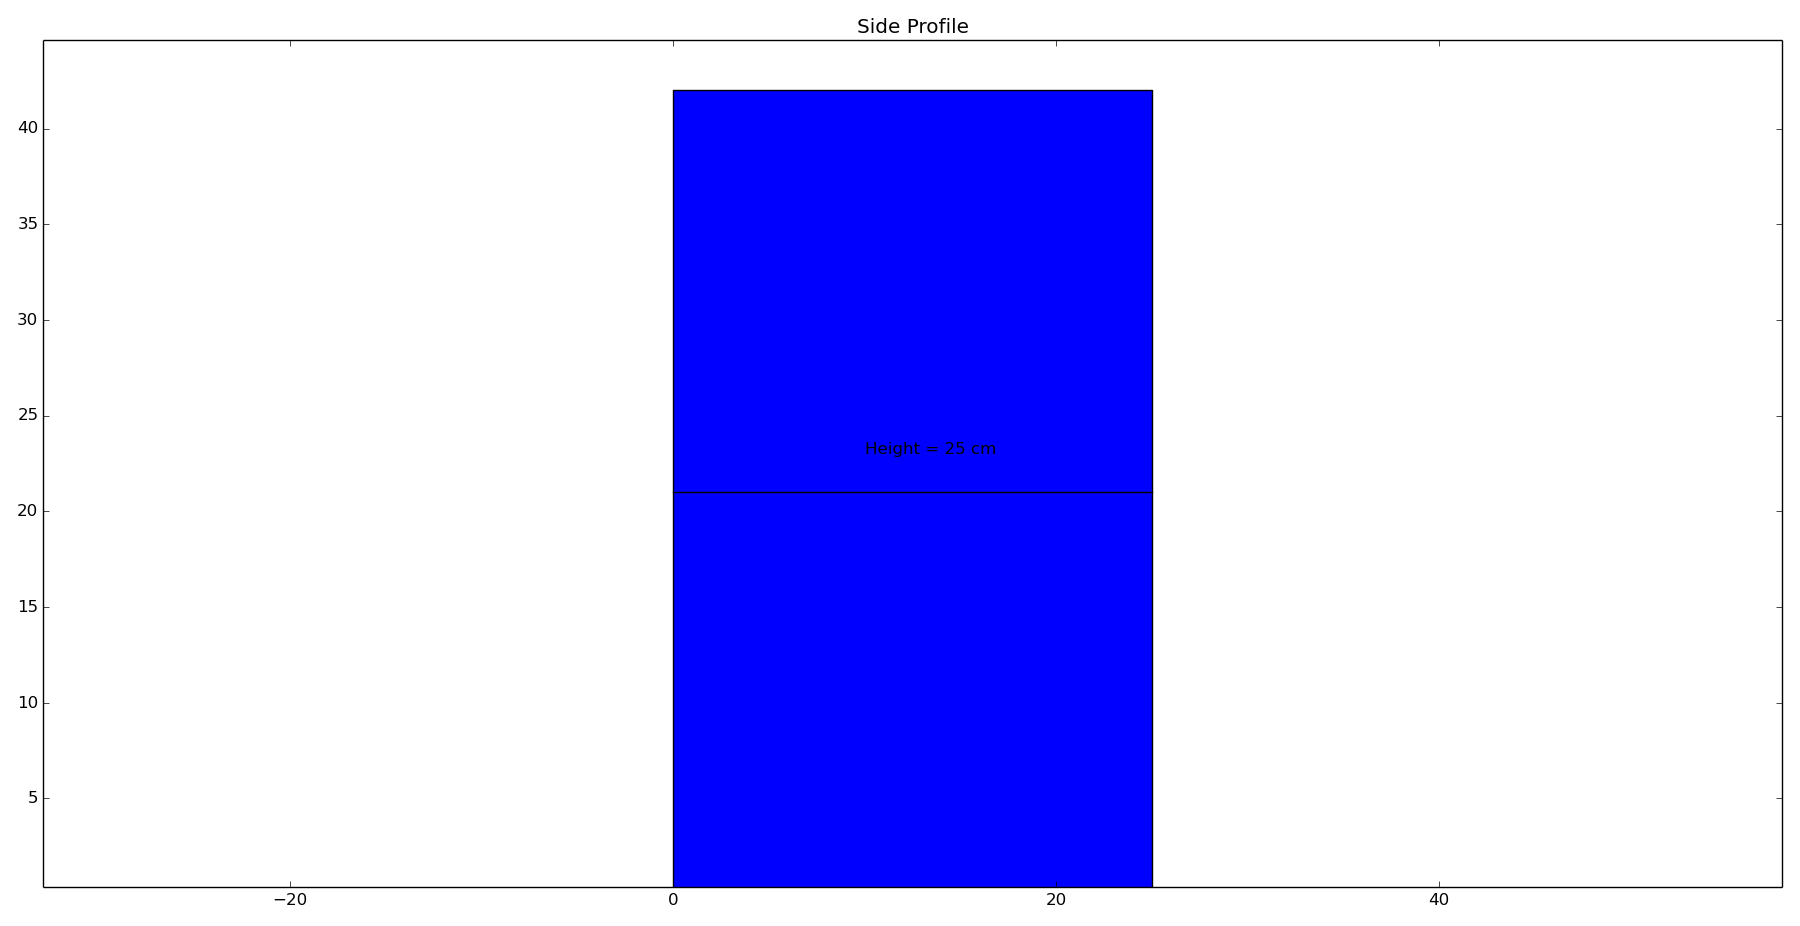
\includegraphics[scale = 0.5]{Figures/Side Profile.png}
    \caption{Side Profile of the cylindrical vessel}
    \label{fig:Side}
\end{figure}

\end{document}
